% !Mode:: "TeX:UTF-8"
\chapter{可见光多波段通信系统概述}
\section{引言}
得益于LED灯在照明市场的风行,使得兼顾通信和照明两重功能的可见光通信技术受到了越来越多的关注。基于LED的可见光通信因其绿色环保、高速便捷、频谱资源不受限制等优点,极有可能在未来的无线通信中占有一席之地,特别是诸如机舱、医院和矿井这些特殊应用场景下。本章将先介绍可见光通信的基本原理,包括基础硬件发光二极管(LED)和光电二极管(PD)的基本工作原理及可见光通信系统模型,然后将概述OFDM在可见光通信中的应用,并且比较ACO-OFDM及DCO-OFDM之间的区别,最后将简介自适应传输技术及其在可见光通信中的应用。
\section{室内可见光通信基本原理}
\subsection{可见光系统模型}
与传统的无线通信技术通过调幅、调频或调相技术将信息调制到射频载波上不同,可见光通信利用的是人眼可见的波长在380 nm到780 nm之间的电磁波来传输信息,并且是使用强度调制(Intensity Modulation,IM)、直接检测(Direct Detection,DD)技术。如\autoref{fig:BasicOpticalSystem}所示,在发射端,利用LED灯的易于调制性,在线性范围内,LED 的发光强度与输入电流功率成正比,将电信号调制到LED发光强度上;在接收端,利用PD的输入反向电流功率与接收到的光强成正比的特性,用光电二极管去检测LED发光强度的变化,将光信号转换成电信号。
\begin{figure}[htbp]
    \centering
    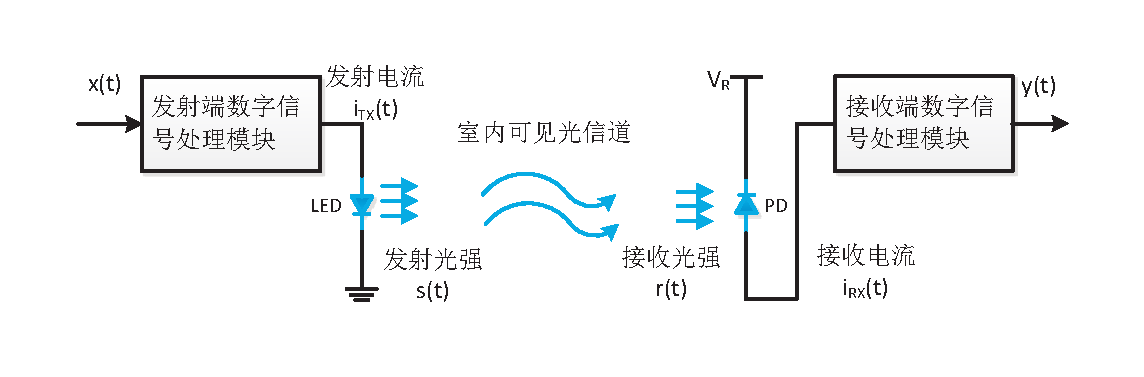
\includegraphics[width=\textwidth]{figures/chapter-2/BasicOpticalSystem.eps}
    \caption{光无线通信系统模型}
    \label{fig:BasicOpticalSystem}
\end{figure}
如\autoref{fig:BasicOpticalSystem}所示,在电信号域(Electrisity domain)发射端输出电压信号$x(t)$经过发光二极管后变成LED的电流$i_{TX}(t)$信号,接收端光敏二极管PD输出电流$i_{RX}(t)$,其最后转换成接收信号$y(t)$ ,在光信号域(Light Domain),首先在发射端发光二极管LED的电流信号$i_{TX}(t)$ 转变为发光强度$s(t)$,经过光信道后,在接收端光电二极管PD收到的光强信号为$r(t)$,经过光电转换,得到电流$i_{RX}(t)$。
所以在实际可见光通信系统中,信号传输由电光变换,光通道传输及光电变换三个过程组成,如\autoref{fig:BasebandModle}所示,接收端信号$y(t)$ 可以表示为:
\begin{equation}
    y(t)=x(t)\otimes h_1(t)\otimes h_2(t)\otimes h_3(t)+z(t)
\end{equation}
其中,$x(t)$表示发射端基带电压信号,$h_1(t)$表示电光转换系统的时域信道冲激响应(Channel Impose Response,CIR),$h_2(t)$表示可见光信道的时域信道冲激响应,$h_3(t)$表示光电转换系统的时域信道冲激响应
\cite{Yangxuecheng2015},
$z(t)$表示信道加性白高斯噪声(Additive White Gaussian Noise,AWGN),符从$z(t)\sim N(0,N_0/2)$分布,$N_0$为其功率谱密度,$\otimes$表示卷积运算。可见光通信系统的噪声,通常主要由热噪声和散弹噪声
\cite{Chenchunyan2014}。热噪声是一种高斯白噪声,在传统的射频无线通信系统中是很常见的。
散弹噪声也可以建模为白高斯噪声来处理,因为两个独立分布的高斯噪声还是高斯的,故我们可以将系统噪声统一建模为与信号独立的高斯白噪声。

\begin{figure}[htbp]
\centering
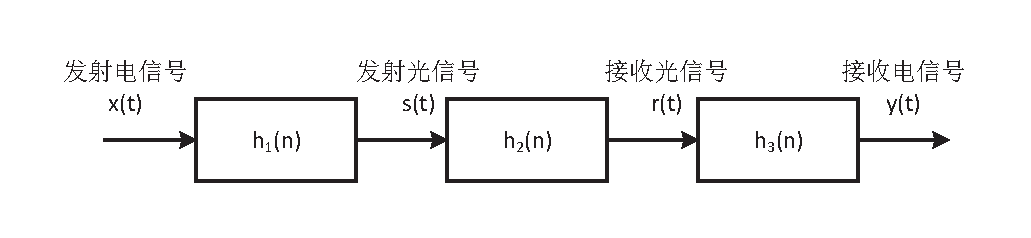
\includegraphics[width=0.9\textwidth]{figures/chapter-2/BasebandModle.eps}
\caption{光无线通信系统基带处理模型}
\label{fig:BasebandModle}
\end{figure}

\subsection{光电元器件简介}
如前文所述,可见光通信与传统的无线通信最大的区别在于调制与信号检测上,射频无线通信必须把基带信号通过调幅、调频或者调相技术调制到高频率的载波上,在接收端再下变频得到基带信号。但目前可见光通信器件技术还不能直接去调制光的幅度、频率或者相位,而是使用发射端强度调制和接收端直接检测技术。在发射端,需要电光转换器件将电信号转换成光信号,在室内可见光通信中用到的主要是发光二极管LED,LED就是调制器,其工作线性范围是一个非常重要的指标,因为如果输入信号的动态变化范围较大,超出LED的线性调制范围,则会发生非线性失真,将严重影响通信性能,在可见光OFDM系统中尤其要注意这点,另外,LED的响应时间是另一个重要指标,响应时间断的LED能够被更高频率的信号调制,也就意味着带宽增加、通信速率增高。在接收端,需要光电转换器件将光信号再变成电信号以进行解调解码,目前大量使用的是光电二极管PD,光电二极管的PN结面积相对比较大,以便接收更多的入射光,其在反向电压的作用下,没有光照时,反向电流非常小,称为暗电流;在有光照时,反向电流急速增大,并且在一定范围内反向电流功率与光照强度成正比。本节将详细介绍发光二极管和光电二极管的通信特性。
\subsubsection{电光转换器件}
目前在光通信领域使用得电光转换器件主要有激光二极管(Laser Diode,LD)和发光二极管LED两类,这两种器件的性质差异很大,应用场景也不同。激光二极管响应速度非常快,但是线性区间非常小,几乎只有关闭和激发两种状态,而且发光角度较小,通信时需要发射端与接收端对准,所以一般用于高速光纤通信中。这里我主要讨论室内无线光通信使用的发光二极管LED。

发光二极管LED是一种掺杂了镓(Ga)、砷(As)和磷(P)等化合物的半导体器件,它跟普通的二极管一样,具有单向导电性,内部有PN节,P区含有多余的电子,N区则有多余得空穴。当给发光二极管加正向电压时,P区的高能电子与N区的空穴结合发生能级跃迁变为低能电子,根据能量守能,其将向外辐射电磁波,并且包含波长在380 nm到780 nm之间的人眼可见的电磁波,具体辐射电磁波的波长主要由掺杂物的种类相关,这就是LED发光的基本原理。

众所周知,白光是一种混合光,故我们日常用于照明的白光LED灯发出的白光也是由几种光合成的。现在市面上的白光LED主要有两种类型。一种是磷光激发型,由蓝光LED激发荧光物质发出黄光,然后蓝光与黄光混合成我们人眼看到的白光;另一种是多色混合型,由多个LED发出不同颜色的光直接合成为白光,这种类型常见的红绿蓝(RGB)LED灯内部就含有三块晶片,分别发红光、绿光和蓝光。\autoref{fig:OSTAR-Spectrum}所示是德国OSRAM公司生产的磷光激发型发光二极管Lighting Plus LE UM S2LN的相对光谱分布图\cite{LE2011},图中峰值位于445 nm处的是蓝光LED发出的蓝色光波,而峰值位于555 \autoref{fig:RGB-Spectrum}所示,其具体型号为LRTB R98G,同为OSRAM生产。图中可见红绿蓝三种色光的峰值分别位于635 nm、525 nm和465 nm处,与林光激发型LED不同的是,红绿蓝三种色光分别由三种不同的LED晶片产生,都有很好的响应速度,我们可以对这三种色光分别调制,达到同时传输三路数据的目的,这样可以大大加大传输速率,即为前文所述的多色白光通信系统。

\begin{figure}[htbp]
\centering
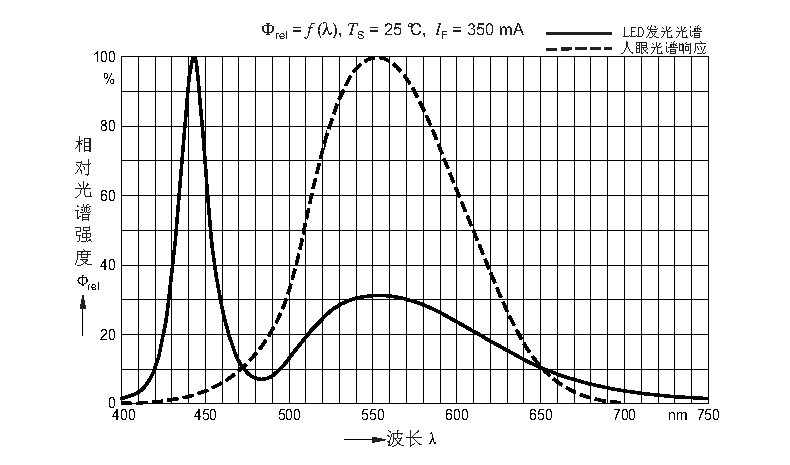
\includegraphics[width=0.9\textwidth]{figures/chapter-2/LEUWS2LN-RelativeSpectralEmission.eps}
\caption{磷激发型LED光谱图}
\label{fig:OSTAR-Spectrum}
\end{figure}

\begin{figure}[htbp]
\centering
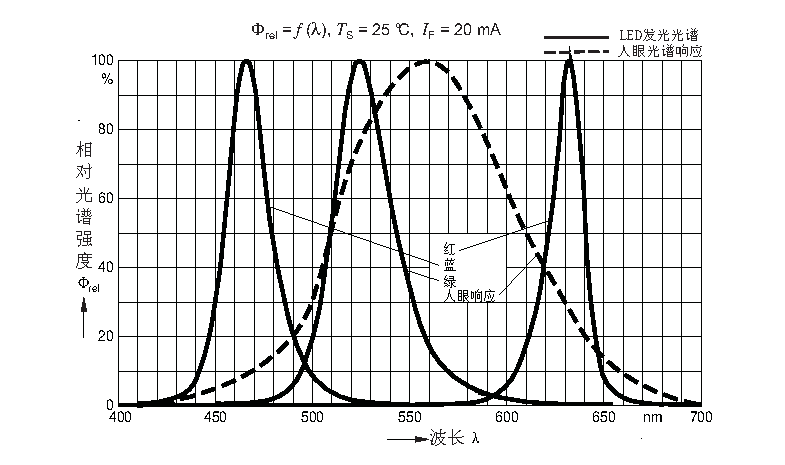
\includegraphics[width=0.9\textwidth]{figures/chapter-2/LRTBR98G-RGB-RelativeSpectralEmission.eps}
\caption{RGB三原色混光型LED光谱图}
\label{fig:RGB-Spectrum}
\end{figure}



\section{OFDM技术在室内可见光通信中的应用}
\subsection{OFDM技术简介}
\subsection{可见光中的OFDM调制}
\section{自适应传输技术简介}
\section{本章小结}
